%%%%%%%%%%%%%%%%%%%%%%%%%%%%%%%%%%%%%%%%%%%%%%%%%%%%%%%%%%
% Ping GCM
%%%%%%%%%%%%%%%%%%%%%%%%%%%%%%%%%%%%%%%%%%%%%%%%%%%%%%%%%%
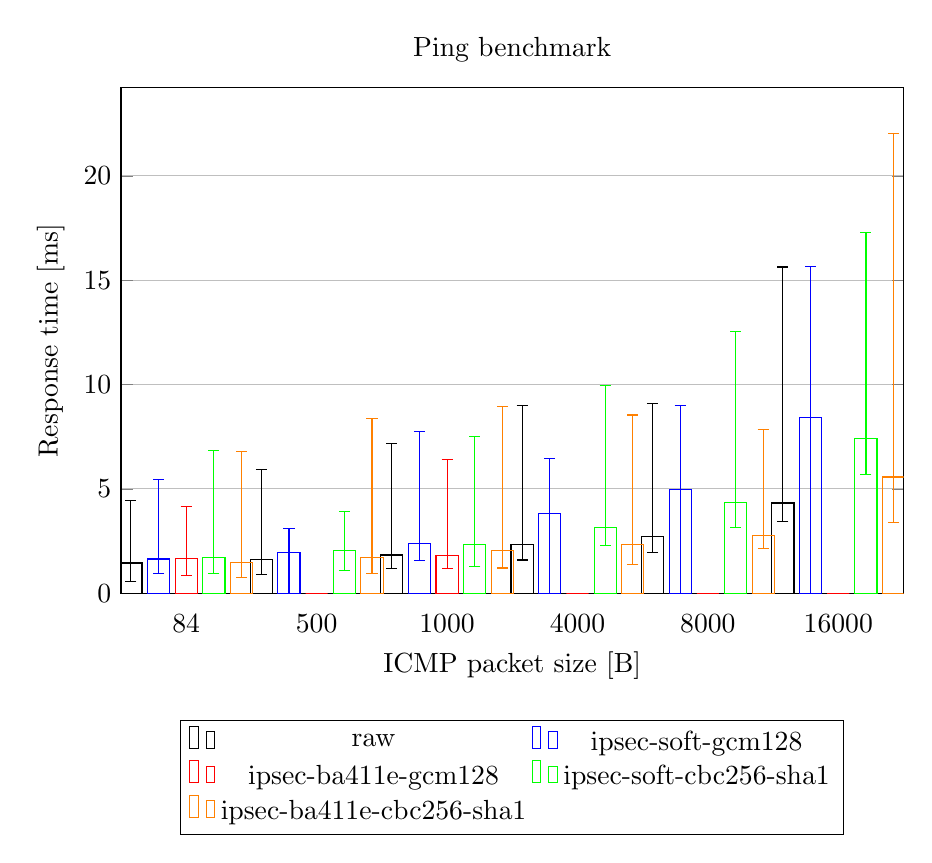
\begin{tikzpicture}
\begin{axis}[
        title = {Ping benchmark},
        width  = 0.95*\textwidth,
        height = 8cm,
        major x tick style = transparent,
        ybar,
        bar width=8pt,
        ymajorgrids = true,
        ylabel = {Response time [ms]},
        xlabel = {ICMP packet size [B]},
        ymin=0,
        symbolic x coords={84, 500, 1000, 4000, 8000, 16000},
        xtick = data,
        scaled y ticks = false,%Disable the *10^4 exponent applied to all y axis markings.
        legend style={at={(0.5,-0.25)}, anchor=north,legend columns=2},
        enlarge x limits=0.1,
    ]
% I would have prefered to have "\addplot[marks only]", but they overlap if they have the same x coordinate,
% not like bars that automatically shift.
\addplot[style={black,fill=none}, error bars/.cd, y dir=both, y explicit]
    coordinates {
        (84,1.448) += (0, 2.983) -= (0,0.899)
        (500, 1.603) += (0, 4.312) -= (0, 0.685)
        (1000,1.832) += (0, 5.324) -= (0,0.661)
        (4000, 2.353) += (0, 6.633) -= (0, 0.76)
        (8000, 2.7) += (0, 6.374) -= (0, 0.746)
        (16000, 4.323) += (0, 11.311) -= (0, 0.892)
    };
    \label{raw}

\addplot[style={blue,fill=none}, error bars/.cd, y dir=both, y explicit]
    coordinates {
        (84,1.640) += (0, 3.806) -= (0, 0.696)
        (500, 1.958) += (0, 1.160) -= (0, 6.945)
        (1000,2.375) += (0, 5.379) -= (0, 0.789)
        (4000, 3.824) += (0, 2.654) -= (0, 10.034)
        (8000, 4.966) += (0, 4.013) -= (0, 12.917)
        (16000, 8.444) += (0, 7.196) -= (0, 16.804)
    };
    \label{ipsec-soft-gcm128}

\addplot[style={red,fill=none}, error bars/.cd, y dir=both, y explicit]
    coordinates {
        (84,1.672) += (0, 2.503) -= (0, 0.8)
        (500, 0) += (0, 0) -= (0, 0)
        (1000,1.803) += (0, 4.608) -= (0, 0.601)
        (4000, 0) += (0, 0) -= (0, 0)
        (8000, 0) += (0, 0) -= (0, 0)
        (16000, 0) += (0, 0) -= (0, 0)
    };
    \label{ipsec-ba411e-gcm128}

% \addplot[style={blue,fill=none}, error bars/.cd, y dir=both, y explicit]
%     coordinates {
%         (84, 1.673) += (0, 6.584) -= (0, 0.623)
%         (500, 2.210) += (0, 6.511) -= (0, 1.087)
%         (1000, 2.377) += (0, 1.181) -= (0, 0.706)
%         (4000, 3.806) += (0, 6.053) -= (0, 0.905)
%         (8000, 5.787) += (0, 12.850) -= (0, 1.616)
%         (16000, 9.006) += (0, 8.848) -= (0, 1.313)
%     };
%     \label{ipsec-soft-gcm256}

% \addplot[style={red,fill=none}, error bars/.cd, y dir=both, y explicit]
%     coordinates {
%         (84, 1.625) += (0, 6.766) -= (0, 0.695)
%         (500, 0) += (0, 0) -= (0, 0)
%         (1000, 2.308) += (0, 5.878) -= (0, 0.797)
%         (4000, 0) += (0, 0) -= (0, 0)
%         (8000, 0) += (0, 0) -= (0, 0)
%         (16000, 0) += (0, 0) -= (0, 0)
%     };
%     \label{ipsec-ba411e-gcm256}

\addplot[style={green,fill=none}, error bars/.cd, y dir=both, y explicit]
    coordinates {
        (84, 1.733) += (0, 5.089) -= (0, 0.789)
        (500, 2.063) += (0, 1.856) -= (0, 0.956)
        (1000, 2.324) += (0, 5.173) -= (0, 1.053)
        (4000, 3.172) += (0, 6.766) -= (0, 0.892)
        (8000, 4.363) += (0, 8.178) -= (0, 1.220)
        (16000, 7.433) += (0, 9.859) -= (0, 1.730)
    };
    \label{ipsec-soft-cbc256-sha1}

\addplot[style={orange,fill=none}, error bars/.cd, y dir=both, y explicit]
    coordinates {
        (84, 1.487) += (0, 5.315) -= (0, 0.731)
        (500, 1.697) += (0, 6.691) -= (0, 0.757)
        (1000, 2.052) += (0, 6.914) -= (0, 0.843)
        (4000, 2.351) += (0, 6.192) -= (0, 0.975)
        (8000, 2.754) += (0, 5.08) -=  (0, 0.61)
        (16000, 5.569) += (0, 16.448) -= (0, 2.194)
    };
    \label{ipsec-ba411e-cbc256-sha1}

% \addplot[style={orange,fill=none}, error bars/.cd, y dir=both, y explicit]
%     coordinates {
%         (84,) += (0, ) -= (0, )
%         (500, ) += (0, ) -= (0, )
%         (1000,) += (0, ) -= (0, )
%         (4000, ) += (0, ) -= (0, )
%         (8000, ) += (0, ) -= (0, )
%         (16000, ) += (0, ) -= (0, )
%     };
%     \label{ipsec-ba411e-cbc256-sha1}

\legend{raw, ipsec-soft-gcm128, ipsec-ba411e-gcm128, ipsec-soft-cbc256-sha1, ipsec-ba411e-cbc256-sha1}
\end{axis}
\end{tikzpicture}
% Here, I could show the gcm128, which show better performances with the BA411e, but I would be weird to compare it with aes256cbc.
% I need another graph with a CPu usage comparison to show that even if the perf are the same for soft/hard with aes256gcm, the hard loads less the CPU (I hope so, at least).